\documentclass{article}
\usepackage[utf8]{inputenc}
\usepackage{hyperref}
\usepackage{amsmath}
\usepackage{graphics}
\usepackage{graphicx}
\usepackage{float}
\graphicspath{ {images/} }
\title{Starlings Murmuration Simulation}
\author{Sankalan Pal Chowdhury, Shreshth Tuli}
\date{April 2018}

\begin{document}

\maketitle

\section{Introduction}
Starlings are a species of small birds that show tendency to migrate in flocks. These flocks are called murmurations and can contain thousands of starlings. Due to their small size and coordinated movements, they can often put up very beautiful displays while moving. In this project, we try to mathematically model this behavior of theirs and run a Computer Simulation of the same
\section{Modeling the Starling}
We seek to model each bird as an individual agent which reacts to its surroundings in order to determine its flying direction. In the most simple model, its environment consists only of other birds. The bird must therefore negotiate three types of constraints in order to determine its flying direction: External forces, Internal forces and Personal limitations.
\subsection{External Forces}
External forces are the forces of mother nature which the bird act on the bird. We assume that the bird does not need to spend energy to generate these forces, and also cannot have any direct control over them. While there are many such forces, we seek to model only the major ones(this selection is similar to what is done for modeling airplanes):
\begin{itemize}
    \item \textbf{Gravity:} Gravity is perhaps the simplest yet most significant force to model. The concept of flight is fascinating essentially since it seems to overcome gravity.
    \item \textbf{Buoyancy:} Buoyancy may not be too important in air, but it is extremely easy to adjust within gravity. It can become significant for birds with very low density, so it cannot harm to model it.
    \item \textbf{Lift:} The  lift force is the main contributor towards overcoming gravity. In fact the bird can maintain its altitude only if the sum of Lift and Buoyancy is same as Gravity.
    \item \textbf{Drag:} The drag force arises due to air resistance which tries to prevent the motion of any body traveling through a fluid. But for this force, the bird could keep flying without applying any effort.
\end{itemize}
Birds, unlike airplanes can flap their wings in order to generate upward force. This force is more like a buoyant force, but needs the bird to spend energy to get it and can also control its magnitude to some extent. Modeling this requires a deep insight of the anatomy of the starlings which is beyond the scope of the model designers, therefore, we do not include it here.
\subsection{Internal Forces}
Once the external forces have been decided, the bird may decide to fly in a certain direction. It is somewhat misleading to call this decision a force, these are actually factors based on which the bird decides what kind of force to apply on itself(actually the bird applies the force on the environment and it gets it force by Newtons Third Law). These, however are all vector quantities and it is rather intuitive to consider them as components of the net force that the bird applies. 

In the current model, we consider three forces, which are commonly used to simulate \href{https://en.wikipedia.org/wiki/Flocking_(behavior)}{flocking behaviour}:
\begin{itemize}
    \item \textbf{Cohesion:} The cohesive force is the attractive force that a bird experiences towards other members of the flock. It ensures that the flock stays together and does not start moving in random directions.
\begin{figure}[h]
\centering
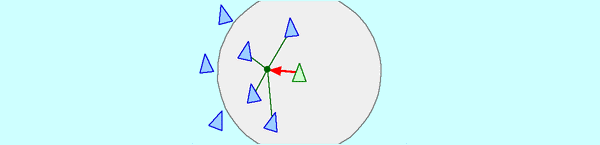
\includegraphics[width=10cm]{cohesion600}
\end{figure}
\item \textbf{Separation:} The separative force acts opposite to the cohesive force and ensures that the birds keep a minimum distance between them and don't start colliding with each other
\begin{figure}[h]
\centering
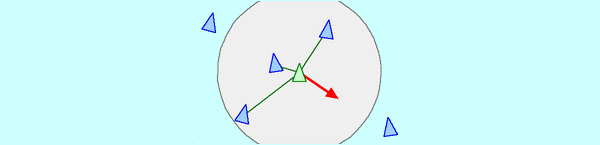
\includegraphics[width=10cm]{separation600}
\end{figure}
    \item \textbf{Alignment:} This force tries to coordinate the direction of motion of the entire flock. Each bird has the urge to fly in the same direction as its neighbors.
\end{itemize}
\begin{figure}[h]
\centering
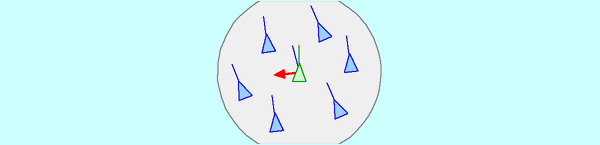
\includegraphics[width=10cm]{alignment600}
\end{figure}

The above mentioned factors present a somewhat idealistic view of how a certain bird desires to fly. However, there are other factors effecting how the bird really flies.

To start off, a bird is not likely to know about another bird which is flying right behind it. In fact, it can only see those birds which are in its \textbf{field of view}, ie the maximum angle from its line of motion which it can see. This is actually quit large for birds since they have eyes on the sides of their heads. Further, two birds which are far off from each other are less likely to affect each other than two birds that are close by. This phenomenon is modeled by the (near)\textbf{sightedness} of the bird. Finally, some birds may be more \textbf{adventurous} than others, giving them urges to fly off in random directions rather than those specified by the above forces.

Finally, a bird can apply only a limited amount of force, in which it would try to overcome the External forces and move in its desired direction. This limit would be determined both by an overall \textbf{maximum acceleration} and the individual \textbf{strength} of the bird.
\section{Mathematical Formulation}
To begin our mathematical formulation, we need to first fix a coordinate system. We fix the origin at the flock centroid(this is beneficial for bounding box creation during implementation) and the y axis upwards. The x and z axis are arbitrarily chosen since the system has cylindrical symmetry.

The mathematical values of the external forces are more or less standard and do not require much explanation
\begin{center}

    $$\vec{F_{gravity}}=\rho_{bird}V\vec{g}$$
    $$\vec{F_{buoyancy}}=-\rho_{air}V\vec{g}$$
    $$\vec{F_{lift}}=C_{lift}\rho_{air}\vec{v}^2W\hat{j}$$
    $$\vec{F_{drag}}=-\frac{1}{2} C_{drag}\vec{v}^2A\hat{v}$$
    $$\vec{F_{external}}=\vec{F_{gravity}}+\vec{F_{buoyancy}}+\vec{F_{lift}}+\vec{F_{drag}}$$

    $$\rho_{bird},\rho_{air} \text{ are the densities of the bird and air,}$$
    $$C_{lift}, C_{drag} \text{ are the lift and drag coefficients,}$$
    $$g \text{ is the acceleration due to gravity }=0\hat{i}-9.8\hat{j}+0\hat{k}$$
    $$W, A \text{ are wing area and cross sectional area respectively,}$$
    $$\vec{v} \text{ is the current velocity of the bird,}$$
    $$V \text{ is the volume of the bird}$$
 
\end{center}

The internal forces are more involved. To begin with, field of view simply filters out the birds which are beyond the specified angle, so all statements made hereafter are w.r.t. the rest of the birds.

\subsection{Internal Forces}
Two different approaches are possible to deal with the sightedness issue. One is to say that only a fixed number of nearest neighbors affect the bird. This partially relies on the fact that the bird would not want to over complicate its life and would approximate the world by a fixed number of birds around it. However, the evidence for this is quite empirical and needs to be judge in light of the fact that the number of birds in a certain region around the bird is held more or less constant by the Cohesion and separation forces. This also does not account for the chance that the bird might look at a very distant bird and adjust itself according to it.

The other view is to limit the distance till which a bird can see. This seems more logical, except for the fact that there is unlikely to be a hard boundary at a given distance. Therefore, we choose an exponential decay function to model the sightedness of the birds:
\begin{center}
$$W_i=e^{-sd_i}$$
\[
    d_i \text{ is the distance to the } i^{th} \text{ bird}
    s \text{is the sightedness of the bird}
\]
\end{center}
At this point, it may seem strange that a bird would look at like a thousand other birds before deciding which direction to move, which is clearly illogical. One way of explaining this would be that the bird looks at only a certain number of birds at each moment, and the quantity mentioned here is the over time expectation of looking at each bird.

This done, we can move on to the three forces. We calculate for each bird separately(call this the target bird and then aggregate to get the net forces.

It is intuitive to keep Alignment proportional to the velocity of the target bird. As for Separation and Cohesion, they should logically be proportional to the inverse of the distance between the two birds(Actually, cohesion can be constant, allowing for the sightedness to take care of the distance factor. Ignoring this fact is more of a personal intuition). Also, the separation force needs to grow faster that the cohesion force, as we want to prevent collisions. We chose to take the simplest expressions that satisfy these constraints.
\begin{center}
$$\vec{F_{cohesion,i}}=\frac{C_{coh}}{d_i} \hat{d_i}$$
$$\vec{F_{separation,i}}=-\frac{C_{sep}}{d_i^2} \hat{d_i}$$
$$\vec{F_{align,i}}=C_{ali}\vec{v_{i}}$$

$$\hat{d_i} \text{ is the unit vector towards the } i^{th} \text{ bird }$$
$$\vec{v_{targ}} \text{ is the velocity of } i^{th} \text{ bird }$$
$$C_{coh},C_{sep},C_{ali} \text{ are respective coefficients}$$ 
\end{center}

Once these forces are calculated due to each bird, we need to aggregate them to get net internal force. Aggregation can be done in many ways, but the two most common ways are summation and averaging. Summation is good for aggregating quantities that are likely to add up destructively. This is clearly true for the separation force. Averaging, on the other hand, make sense for quantities that would add up constructively, like the alignment force. Cohesion force can go either way, but it is somewhat safer to consider averaging since a zero is less dangerous than an infinity. The Weights assigned to the different birds is taken care of here.

\begin{center}
    $$\vec{F_{cohesion}}=\frac{\sum_iW_i\vec{F_{cohesion,i}}}{\sum_iW_i}$$
    $$\vec{F_{alignment}}=\frac{\sum_iW_i\vec{F_{alignment,i}}}{\sum_iW_i}$$
     $$\vec{F_{separation}}=\sum_iW_i\vec{F_{separation,i}}$$
\end{center}

Finally, we need to add the adventure component to these forces to calculate the net internal force on the bird. Now, while an adventurous bird may not want to align itself with the other birds or get attracted to them, it will certainly not want to collide with other birds. Therefore, the random component will only replace the alignment and cohesion forces and not the separation force.
\begin{center}
    $$\vec{F_{internal}}=\vec{F_{separation}}+\frac{1000-Adv}{1000}(\vec{F_{cohesion}}+ \vec{F_{alignment}})+\frac{Adv}{1000}\vec{R}$$
    
    $$Adv \in \{0,...,1000\} \text{ is the adventurousness parameter }$$
    $$\vec{R} \text{ is a suitable random vector(suitability depends on range of magnitudes)}$$
\end{center}
\subsection{Putting it Together}
Now that we have both the external and internal force vectors, we need to put them together to calculate the acceleration, velocity and power of the bird. It is here that we need to take into account the maximum force that the bird can apply is limited.

If the bird was an inanimate object, it would simply drift in the direction of the external force. What the bird really does is try its best to change this to its desired direction of flight as much as possible. This difference is simply given by $\vec{v_{diff}}=\vec{v}+\vec{F_{external}}-\vec{F_{internal}}$. Since we can only take discrete time, the desired acceleration is $\vec{a_{desired}}=\vec{v_{diff}}/P$ where P is the clock period. The magnitude of  $\vec{a_{desired}}$ needs to be bounded by a $a_{bound}=a_{max} \times strength$ where $a_{max}$ is the global maximum acceleration and strength is a property of the bird.\newline

The bounding mechanism itself is somewhat non trivial. The naive way of doing it would be to cut off any value higher that the required bound. But that would be very unrealistic as in a real scenario, the bird would start facing difficulty gradually till it reaches a point where it can no longer fly faster. 
A good function to approximate this is the $tanh$ function, which has derivative of 1 around zero, but is bounded by 1 on the positive side. However, its derivative never falls to 0 for any finite parameter.

Once the bounding is done, we can calculate Power easily using laws of physics.
\begin{center}
    $$\vec{a_{final}}=tanh(\frac{|\vec{a_{desired}}|}{a_{bound}})\frac{a_{bound}}{|\vec{a_{desired}}|}\vec{a_{desired}}$$
    $$\vec{v_{final}}=\vec{v}+\vec{v}+\vec{F_{external}}-\vec{a_{final}}$$
    $$Power=m\vec{a_{final}}.\vec{v_{final}}$$
\end{center}
Position and Energy follow trivially.


\pagebreak
\section{Implementation}
Having designed the model, we attempt to implement it on a computer. The aim of this part is to 1) Be able to visualize the murmurations of the starlings on a computer screen, and 2) approximate some statistics about these murmurations.

The implementation needs to proceed in two parts. First, we look at what kinds of deviations must be made from the original model in order to be able to simulate it. Second, we choose a framework to implement the design. Both of these are dependent on the characteristics of the model and/or the constraints set by the programming environment.
\subsection{Deviations from the Model}
One of the major issues we need to deal with here is the fact that in real life, Starlings are free to move anywhere in the open sky. However, our simulation only lets us look at the starlings from a fixed viewpoint, and there is little point in having the murmurations happening out of the visible region. There are multiple options to solve this:
\begin{itemize}
    \item \textbf{Moving the Viewpoint:} This approach tries to approximate the real motions of the birds as best as possible, by moving the viewpoint automatically along with the birds. The main advantage of this is the model does not need to be tampered with. However, there can be scenarios in which the motion of the view point would cancel out the motion of the birds, making them appear to be static. Also, the flock may split into two, leading to issues on deciding the viewpoint. Alternatively, the shifting of viewpoint can be left upto the user, but that is probably not very user friendly.
    \item \textbf{A Circular World:} To give the feeling of an infinite space, we can make the edges of the view wrap around to the opposite edge. This also would require minimal changes to the model, but its physical effect can hardly be explained. Also, it is not logical anyway to let the $-y$ direction extend to infinity.
    \item \textbf{Adding Imaginary Force}: To prevent the birds from escaping into infinity, we can define a potential like field that forces the birds to remain in a specified region, beyond which this field becomes too large. This can represent pressure zones or simply unfamiliar territory for the birds. However, if not tuned properly, such a field can cause the birds to actually divert to infinity.
    \item \textbf{Limiting Position Directly:} This would be similar to what was done for limiting the maximum acceleration, forcing the birds to stay in a fixed region. The chief downsides of this is the lack of a physical explanation and the fact that the birds might all want to escape in one direction, but get restricted by this force, making them appear as if they are all at the same point.
\end{itemize}
In our current implementation, we choose to go with a combination of the last two approaches, which tend to cancel out some of each others negative points. For the force field, we choose a force that is zero in some region around the origin and then grows as the square root of distance from origin. This choice is kind of empirical, with comparisons performed over multiple regularized polynomial fields. The modified set of equations are given below:
\begin{center}
    $$\vec{v_{positional}}=-\vec{P} * max(\sqrt{\frac{|\vec{P}|}{P_{max}}}-\sqrt{5},0)$$
    $$\vec{v_{diff}}=\vec{v}+\vec{F_{external}}-\vec{F_{internal}}-\vec{v_{positional}}$$
    $$\vec{P_{final}}=tanh(\frac{|\vec{P_{desired}}|}{20*P_{max}})\frac{20*P_{max}}{|\vec{P_{desired}}|}\vec{P_{desired}}$$
    P \text{represents position of the bird, no subscript means current position}
\end{center}
The other equations remain unchanged.
Apart from this, it turns out that the exponential sightedness model can sometimes become too much to calculate(it needs to be done O($n^2$) times in each time step, where n is the number of birds). We therefore keep an alternative of using a constant viewing range(ie a step function). In the same vein, all the other internal forces are also made toggle-able. 

\subsection{Frameworks and Design Decisions}
While it has not been stated previously, some decisions are implicit to our model:
\begin{itemize}
    \item Since every starling has been modeled as an entity, and \textbf{Object Oriented Paradigm} is necessary to implement these.
    \item there is a stochastic dimension to this simulation. Every calculation therefore need to be performed on a clock edge.
    \item Interaction between different birds is purely observational, so the all the computations are parallelisable. This makes our program fit for multi-threading.
\end{itemize}
\subsubsection{The Clock}
While it is clear that a clock needs to be used, there are actually multiple options on how the clock gets used. The simplest way to go about it is to use a \textbf{real clock} which calculates the position and updates the display in real time. In such a setting, there would be a trade off between the frequency of the clock and the number of birds. The advantage, however is that no storage needs to be done in order to create a realistic display.

The alternative to this approach is to use a \textbf{logical clock} which can proceed at much slower pace than the actual clock, which only influences the display. This means that we can slow down the Logical clock arbitrarily, allowing us to simulate as many birds as we like(well, kind of). In such an approach, the user cannot dynamically set parameters or visualize what the current setting looks like. The main problem here though, is the fact that the positions of each bird needs to be saved into a file, and this file can get huge. 

Suppose we store the position and velocity of each bird at each instant as vectors of single precision floats. If we use a 50 hz clock for 2000 birds for 10 minutes we end up with $50*6*1000*30*32=1.152 Gb$ of data. Note that this data would not make any sense to a human, and if we want to use a text file, the file size blows up even more. Another consideration here is that the display of the birds itself takes up significant computational power, and that needs to be done on a real clock anyway. 

Therefore, we choose to stick to a real clock
\subsubsection{Order of Computation with Multi-threading}
When talking of objects, the ideal model is that all instances of an object run their computation concurrently. This would also be closest to the real world. 

In a real programming paradigm, however, to run everything concurrently is not possible(unless we have as many logical cores as birds). The closest we can get is to give each bird its own thread, but that would mean a huge number of context switches, and therefore huge slowdown. Intuitively, since the steps taken by each bird in each tick of the clock would be rather small, imposing a fixed order should not harm the model too much. 

In our implementation, we use 4 threads(this number can be increased depending on how many cores are available) and within each thread, we provide two options: In one, we impose a fixed order of execution amongst the birds, while in the other, we randomize within each thread. For the non-random approach, a simple segregation scheme is used viz that from the vector of birds thread $t$ gets birds which have index $i$ such that $i\,\%\,4\,=\,t$. Order between the threads is always random, as long as at least 4 cores are available. So there are two levels of randomization that this approach provides:
\begin{enumerate}
\item The inherent scheduler of the operating system and the seemingly random distribution of load on the physical cores, randomize the order in which the computation is done for each bird.
\item An array of numbers 1 to flock size is shuffled and divided into 4 sub-arrays. Each thread gets a sub-array and uses it's values as indices for execution of the computation, thus making it random.
\end{enumerate}

Although the approach used still does not allow concurrent calculation for each bird (which is a limitation of the hardware) but provides the best way to model the system with finite logical cores.
\begin{figure}[H]
\centering
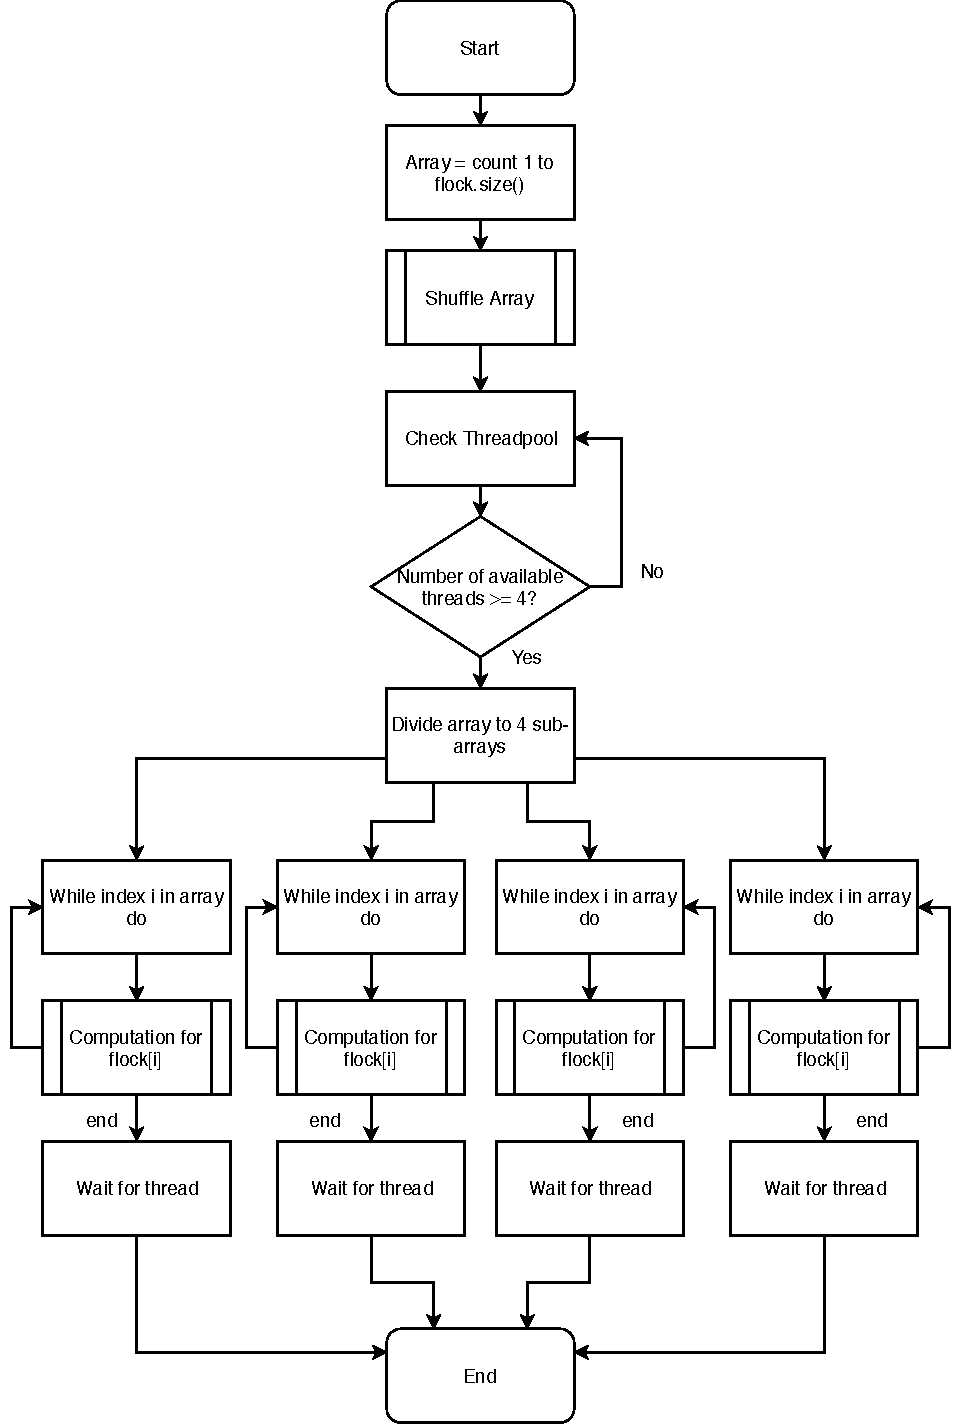
\includegraphics[width=10cm]{Flock_threading}
\caption{Multi-threading flowchart with randomization}
\end{figure}


\subsubsection{Selected tools}
The calculation is implemented in \textbf{C++} because it is perhaps one of the most widely used, rapidly evolving and fastest language for Object Oriented Programming. The display part is done in \textbf{OpenGL} which is said to be the \textit{industry standard for high performance graphics}. Other platforms like $Unity$ and other similar physics engines have not been used as they do not allow tuning at the root level even though they allow users to model the problem much more easily.
\section{Evaluation and Parameter Tuning}
Once we have implemented our design, we need to tune the hyper-parameters in order to get realistic displays. But before that, we need to have some metrics to evaluate the performance.
\subsection{Metrics for Correctness}
In the age of big data and machine learning, one is always talking of differentiable and convex cost functions. Luckily or unluckily, these things have not yet invaded the lives of the starlings, so we need to have heuristic measures of correctness.

The best judgment is obviously given by visualization of the simulation, to judge whether it is realistic or not. However, is is normally better to have a more quantitative measures. Following are some such possibilities:
\begin{itemize}
	\item The most important correctness indicator is the \textbf{visual effect} created by the starlings when in motion. A low number of birds may not give such an effect so relaxation should be for starlings when they are less than say 100.
    \item The starlings have a diet consisting fruits and insects. Based on this, we can estimate how much Energy they can actually spend in flying. Thereafter, we can check if the \textbf{Average Energy} and the \textbf{Maximum Energy} spent by the starling is around this value or not
    \item Based on the energy consumption in a finite time like 10 minutes, the amount of \textbf{food intake} should be less than the typical food intake of a starling in a day which is around 10g. Such measurements are from online sources like \href{https://www.tandfonline.com/doi/pdf/10.1080/00063657309476384}{this}.
    \item The starlings can withstand only so much \textbf{force} on themselves. If it becomes too high, the will probably get squashed. 
    \item \textbf{Collisions} never take place in the real setting, so even if two birds get too close, we should rethink our model. 
    \item The starlings can not apply a large amount of power while in motion, so the parameters \textbf{Average Power} and \textbf{Maximum Power} should be in an acceptable range.
\end{itemize}
Beyond these, there are things like maximum velocity and acceleration, but that have already been accounted for explicitly in our model, so it makes little sense in measuring them. Finally, we should also see what is the maximum number of birds that we are able to simulate, as that is definitely a measure of performance.

\pagebreak

\subsection{Tuning the Hyper-parameters}

Tuning the hyper-parameters is crucial for a more realistic simulation. Although, these parameters can be determined by complex calculations and analysis of the birds anatomical structure and the cognitive model. This becomes much more complicated when such functions are to be mapped for discrete time. A not so precise but more effective approach would be to augment the model parameters by brute-force and intelligent guesses based on the metrics of correctness as discussed earlier. This approach leads to errors in the model, but the deviation from realism is also because of modeling constraints as discussed. These approximations and relaxations allow us to take such a decision for parameter tuning. \\
For the internal forces, the parameter tuning has been based on a intuitive notion of prioritizing the various forces: separation, alignment and cohesion. As separation must dominate at lower distances and cohesion at higher, it is important that the constants used for cohesion are higher than that of separation but the dependence with distance must rise faster in the latter case. For realistic simulation, it is also important to give some randomness to the forces considering that these random forces do not dominate over the systematic ones used in the model. As these forces are based on a factor that exponentially decays or as a step function with distance, there constants must be considering the distances as well. \\
For the external forces including lift, drag, buoyancy and lift some physical aspects need to be investigated. The cross section area and the drag coefficient in the real scenario change dynamically but for the ease of implementation and their somewhat low effect on the model have been neglected. It is important to observe that the drag force depends on the airflow around the bird. A turbulent airflow is expected most of the times due to the flock around it. Thus, we use a drag coefficient somewhat in between but more the side of that for turbulent air. The decision as to how much the air is turbulent or laminar is based on quantitative data of the Reynolds number on the internet as on \href{https://aip.scitation.org/doi/abs/10.1063/1.4807064}{"this"}  link, and empirical observations. 

\section{Conclusion}
In this project we have been able to approximately simulate the murmurations of starlings and also calculate some essential parameters of the motion. The fact that our outputs actually look realistic is definitely evidence in favour of the fact that the real model of flight is somewhat similar to the one that we have defined. This is therefore also a step towards understanding the behavior of starlings.

Finally, our model contains a lot of hyper parameters, thus a lot of flexibility. In future, should someone be able to track the actual motion of starlings, the birds can also be made \textit{Reinforcement Learning} agents.
\end{document}

